\section{Introduction}
Elastic LLM serving releases idle instances to save resources, but capacity
returns only after startup. Queues, running work, and lifecycle transitions
then shape subsequent control decisions. A simulator used to evaluate such
policies must capture when capacity is available, not just how long individual
requests take or how many GPU seconds a run consumes.

FidelityLoop studies these requirements as a closed loop from prediction to policy
decision to physical lifecycle execution. In 36 preregistered runs, the calibrated
replay improves matched-request timing yet worsens occupied-resource
prediction under the same hysteresis rule (H). A startup-endpoint contrast locates
one feedback path at the controller's cooldown boundary, while trajectory
analysis shows that equal total occupation error can hide different control
inputs. We then train PPO policies in replay under two startup-time assumptions,
freeze five checkpoints, and evaluate them against an always-on two-GPU reference.
This 32-cell campaign uses the same registered Qwen/A100 serving stack under a
separately re-provisioned runtime lock to test whether predicted feasibility
survives physical execution. A further six-checkpoint screening study tests
whether the better-performing replay model remains useful for new candidates;
its false rejections expose a limit that aggregate agreement alone misses.

The paper makes three contributions:
\begin{enumerate}[leftmargin=*]
\item \textbf{A closed-loop evaluation framework.} FidelityLoop separates the policy
adapter from lifecycle execution and aligns causal observations, request
identities, lifecycle generations, resource trajectories, and deadline-aware
cost ledgers. The same contract runs fixed rules and learned checkpoints, with
failed requests retained in the denominator.
\item \textbf{A lifecycle-fidelity diagnosis.} Held-out physical runs distinguish
local-service, aggregate-resource, and trajectory fidelity. Event-level
comparisons explain a startup-related divergence and show why aggregate resource
error is insufficient for a closed-loop evaluator.
\item \textbf{A reproducible policy evaluation.} A guard for pending offline deadlines quantifies the
resource--latency trade-off, and the continuous E2 campaign tests five frozen
PPO checkpoints under two arrival regimes. A follow-up screening study exposes
false rejections of feasible new checkpoints. These cases test both policies
and their evaluator:
lower scenario cost is not a saving when deadlines are missed.
\end{enumerate}
The source release provides CPU interface checks and a standalone fixed-event
cost verifier; the supplement maps these checks to their evidence.

\section{Background and motivation}
We consider mixed online and offline LLM workloads served by a limited GPU
pool, where elastic scheduling aims to reduce resource use while meeting
request deadlines. Evaluating every candidate policy on physical hardware
is costly, motivating a framework for replay-based policy development and
training followed by physical validation. FidelityLoop connects these stages
through a shared policy interface and consistent lifecycle and deadline
accounting, so that savings predicted in replay can be checked against
deployment outcomes.

Our exploratory deployment revealed why this connection matters: the calibrated
replay reduced prediction error for matched local requests while
increasing error in occupied GPU time under dynamic scheduling.
These preliminary observations motivate the preregistered study;
they are not additional held-out repeats.

The lifecycle diagnosis separated the old 69.219 s startup proxy from the earlier
window launch-to-ready (25.19 s) and setup (46.80 s) contexts. When the proxy
crossed the 60 s cooldown boundary it changed a target decision, motivating the
locked sequence of calibration, lifecycle checks, and held-out feasibility tests.

Figure~\ref{fig:motivation} summarizes the lifecycle boundary. It is a motivating
diagnostic, not a post-hoc selection rule: the held-out windows were selected once
from the registered forward pool and were not replaced after observing performance.

\begin{figure}[t]
\centering
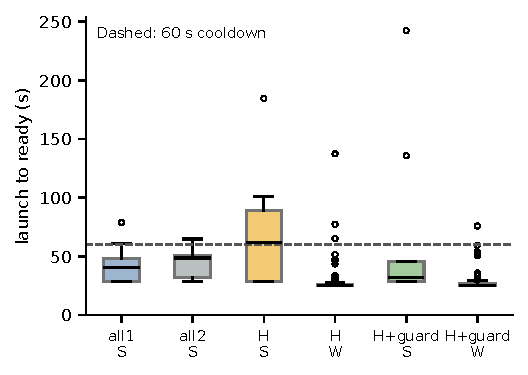
\includegraphics[width=0.98\linewidth]{figures/fig1_lifecycle.pdf}
\caption{Observed startup times in the held-out runs. Labels use S for setup and W
for window scale-out. The dashed line marks the 60-second controller cooldown;
boxes summarize observed launch-to-ready times. Release and cleanup are separate
ledger events. Collapsing these contexts into one endpoint can alter closed-loop actions.}
\label{fig:motivation}
\end{figure}

\section{Related work}
Vidur and Charon use performance simulation to guide LLM configuration choices;
Clockwork studies predictable request timing
\citep{vidur2024,charon2026,gujarati2020clockwork_arxiv}.
FidelityLoop complements these efforts with a shared policy interface for replay
and physical execution, aligning request identities, lifecycle trajectories, and
deadline-aware resource ledgers. This lets us test whether better service-time
fit also improves resource prediction and policy feasibility.

Physical serving systems change how capacity becomes available: cold-start
characterization and systems such as ServerlessLLM expose this lifecycle cost
\citep{kabakibo2026coldstart,fu2024serverlessllm}. We hold the engine and loading
path fixed, changing only simulated timing in the endpoint comparison.

Provisioning and scheduling work connects workload estimates to SLOs
\citep{crankshaw2018inferline,zhang2019mark,zhang2023shepherd}. 
FidelityLoop provides a shared evaluation contract for such policies,
connecting replay predictions to physical execution and deadline-aware
resource accounting. The guard serves as a rule-based case study;
frozen PPO checkpoints extend the evaluation to learned policies.

Policy design provides a complementary layer. Llumnix dynamically reschedules
LLM requests \citep{sun2024llumnix}; AAPA predicts scaling needs for serverless
workloads \citep{zhang2025aapa}; KIS-S learns GPU-inference autoscaling with PPO
\citep{zhang2025kiss}. We use PPO as a
frozen policy family rather than proposing a new RL algorithm; PPO is the
standard clipped policy-gradient method \citep{schulman2017ppo}. Our question
is whether a learned checkpoint selected in replay remains feasible after the
lifecycle backend and deadline ledger are applied.

\section{Problem and metrics}
The system has two accelerators, online arrivals with a 60 s deadline, and 120
offline jobs per 2,100 s observation window with a 300 s deadline. Online requests
run locally or use a delay-only synthetic API sink; offline jobs run locally.
Arrivals span 1,800 s; execution and accounting continue for another 300 s
to cover the remaining deadline horizon.
The primary window cost, in scenario USD, is
\begin{equation}
 C = .001 G + .002 S + .001 D + 10^{-6} I + 3\!\times\!10^{-6} B + .01 M,
\end{equation}
where $G$ is occupied GPU seconds, $S,D$ are starts and shutdowns, $I,B$ are
synthetic API input and output budgets, and $M$ counts offline deadline misses,
including unfinished requests whose deadlines have passed. Setup and cleanup are reported separately and are not folded into the
primary model gate.

Completed means a recorded completion by the observation cutoff; it may be
\emph{on time} (finish time $\leq$ deadline) or \emph{late} (finish time $>$
deadline). An unfinished request has no completed terminal by the cutoff.
Unfinished or censored work is retained in the arrival denominator. The capacity
gate $G_F$ requires all2 (two GPUs throughout) to complete every online and offline
request on time. P1 requires 120/120 offline requests on time, at least 99\%
online requests on time, and no unfinished request; P1+ additionally requires
every online request on time. P2 is a ratio-of-means saving against all1 (one GPU throughout) computed
within each window and then averaged equally across the three windows.

\section{Workload construction}
Online arrivals in the main study come from the successful-request subset of BurstGPT, a public
trace of production LLM requests \citep{wang2024burstgpt}. We read all 1,404,294
source rows and retain source hashes and row identities. The trace has no
session identifier, so the split separates arrival times rather than sessions.
Locally routed requests execute actual GPU inference with fixed-corpus prompts
and registered token budgets. The experiment reproduces arrival-time patterns,
not the original users' prompts or semantic tasks.

The three held-out windows are selected once from the forward pool after the old
windows plus a 30-minute protection band. A 60 s morphology filter defines the
steady, recovery, and burst-offline classes (even, declining, and bursty online
arrivals); a fixed SHA ordering takes
the first eligible candidate in steady--recovery--burst order, subject to the
registered separation constraint. Online rows are thinned with the inherited C2
integer threshold, while the 120 offline jobs are constructed at fixed 15 s
spacing and 256-input/256-output token budgets. The two salts and all thresholds
are fixed in \texttt{s4\_generation\_lock.json}; generated inputs are locked before replay
and never replaced to improve a result.

Table~\ref{tab:workload} reports the arrival shape at the registered 60 s scale.
The 1 s diagnostics are retained in the manifest but do not define the class.
The values describe the selected derived windows, not the full source population.

\begin{table}[t]
\centering
\fontsize{8.5}{10}\selectfont
\caption{Selected window arrival shape at 60 s bins. Each cell is raw/derived;
CV and peak-to-mean use the full 1,800 s window, including empty bins.}
\label{tab:workload}
\setlength{\tabcolsep}{2pt}
\par\vspace{4pt}
\begin{tabular*}{\linewidth}{@{\extracolsep{\fill}}lrrrr@{}}
\toprule
Window & arrivals & CV & peak/mean & lag-1\\
\midrule
steady & 5461 / 1444 & 0.378 / 0.412 & 1.566 / 1.641 & 0.772 / 0.797 \\
recovery & 1141 / 334 & 1.444 / 1.452 & 3.550 / 3.862 & 0.906 / 0.892 \\
burst-offline & 663 / 177 & 1.951 / 1.935 & 6.652 / 6.780 & 0.810 / 0.754 \\
\bottomrule

\end{tabular*}
\end{table}

The derived windows preserve arrival timing and fixed work accounting, but they
are late-source slices with no session fields. They therefore represent a
controlled workload domain for lifecycle decisions, not a claim about all
production traffic or user intent.

E2 uses two separately generated and locked windows from the same
construction pipeline, with no row overlap with the three held-out windows;
the campaigns remain distinct and are never pooled. The recovery window contains 358 derived online arrivals and
120 fixed offline arrivals (478 total); the steady window contains 944 online
and 120 offline arrivals (1,064 total). Offline arrivals are spaced every 15 s,
with 256 input and output tokens; the online rows retain their locked arrival
timestamps. The window identities and input hashes are bound in the E2 lock.

A separate external-validity study uses Azure conversation arrival traces
associated with Splitwise \citep{patel2024splitwise}; its workload construction
and load-boundary results are reported in the supplement.

\section{Experimental setup}
The preregistered held-out study used two NVIDIA A100
80GB PCIe GPUs at \experimentfacility{}, with one independent
tensor-parallelism-1 instance per GPU and Qwen2.5-7B-Instruct. The serving stack
was vLLM 0.9.0 \citep{kwon2023vllm} with PyTorch 2.7.0+cu126, Transformers 4.51.1, tokenizers 0.21.1,
and NumPy 1.26.4. Instances used FP16, maximum model length 4096, maximum batched
tokens 16,384, maximum sequences 1,024, four local request slots, chunked prefill
enabled, prefix caching disabled, eager execution enabled, and GPU memory
utilization 0.8. Readiness required the per-process health probe and the dual-ready
barrier; cleanup required verified process release on both devices. These values are
bound by each run's environment snapshot and GPU identity record.

The held-out study and E2 both use two A100 GPUs. Before held-out execution, the deployment-adapted model (E)
had its lifecycle parameters calibrated and frozen. The historical V--E comparison spans different
hardware environments (A800 and A100), so it does not isolate the
effect of calibration.

The E2 campaign instantiated the same registered Qwen2.5-7B-Instruct serving
stack on two A100 GPUs through the framework contract. It contains 32
locked cells: one all2 capacity anchor and five frozen PPO arms per window, with
three repeats per comparison arm across recovery and steady windows. The campaign
was run under a new runtime lock, with each checkpoint and tensor identity bound
into the result package. It is a policy-execution test, not a model-selection
search or a claim of universal PPO superiority. An earlier 38-run campaign, termed Bridge, evaluated rule-based,
guarded, and PPO policies under a separate runtime lock; its results
are retained as supplementary evidence and are not pooled with E2.
The follow-up screening study (E3) uses six previously undeployed checkpoints
on the same two windows. Each window runs on a separate dual-A100 allocation
with the registered serving stack: one all2 anchor and two repeats per arm,
26 cells in total. E3 is analyzed separately from E2 and Bridge.

\section{Method}
Predictive replay and physical execution share a policy contract. Adapters read
observable queues and device states and
return capacity targets; the guard may also select dispatch priority. The backend
handles readiness, draining, and verified release, while request identities align
predictions, decisions, lifecycle states, resources, and costs. The resulting data
flow is \emph{workload rows $\rightarrow$ causal observation $\rightarrow$ policy
adapter $\rightarrow$ lifecycle backend $\rightarrow$ identity ledger}. A separate
CPU verifier recomputes feasibility and cost from raw records.
By default, ready local slots serve online requests before offline jobs.
Online requests still waiting 10 s after arrival can enter the synthetic API
sink, which admits up to eight concurrent requests and completes each on a
5 s timer. The guard can prioritize at-risk offline jobs; PPO changes capacity
while retaining the default dispatch and API rules.

In the frozen physical stack, the queue-target, predictive, and
queueing-capacity baselines each use 23--38 policy-specific code lines
and share a 73-line adapter and support layer. The supplement separates
policy logic, integration code, and reused dependencies for these
baselines, the guard, and PPO.

The CPU framework exposes interfaces for replacing performance
estimators and policies. On small synthetic
workloads, four historical policy configurations preserve requests, events, and
ledgers exactly, and two device/slot configurations pass conservation checks.
Complementing these interface tests, causal event replay reconstructs observations
and policy state and reproduces all 29,580 logged decisions from 16 earlier
same-runtime runs (supplement). This validates decision reconstruction under
recorded events; prediction fidelity is evaluated separately below.

\subsection{Calibrated models}
The replay models share an executor but differ in service and lifecycle timing
(Table~\ref{tab:replay-model-parameters}). O uses an equal-share service model
and an assumed 30\,s startup. C uses a measured service lookup and a historical
69.219\,s startup proxy; C30 restores the 30\,s assumption. E combines the
lookup with deployment-adapted lifecycle parameters; V retains a bounded
refit from the earlier environment. O--C30 isolates the service model,
whereas C--C30 isolates startup; O--C changes both.

\begin{table}[t]
\centering
\small
\caption{Frozen replay parameters in seconds, rounded to three decimals.
All models share a 69.363\,s setup proxy outside the primary window ledger.}
\label{tab:replay-model-parameters}
\setlength{\tabcolsep}{3pt}
\par\vspace{4pt}
\begin{tabular*}{\linewidth}{@{\extracolsep{\fill}}llrr@{}}
\toprule
Model & Service & Startup & Shutdown\\
\midrule
O & equal-share & 30.000 & 7.059\\
C & measured lookup & 69.219 & 7.059\\
C30 & same lookup & 30.000 & 7.059\\
E & same lookup & 33.497 & 2.224\\
V & same lookup & 25.196 & 2.325\\
\bottomrule
\end{tabular*}
\end{table}

O assumes 1024 input and 128 output tokens/s, shared equally among concurrent
requests. The calibrated lookup uses median measured wall times per
input/output/concurrency cell, interpolating in input length and concurrency
(one to four requests per instance). Its values are shared by C, C30, E, and V.
The supplement's Replay model specification section details measurement sources,
interpolation, and lifecycle fitting. Model bytes, tokenizer, workload identities,
and the candidate grid are locked before held-out execution.

For each model prediction and physical repeat of a window, the dimensionless
lifecycle loss is
\begin{equation}
 L=\frac{0.5|\Delta G_{\rm occupied}|+0.25|\Delta G_{\rm active}|}{2T}
   +\frac{0.25|\Delta Q|}{TN},
 \label{eq:lifecycle-loss}
\end{equation}
Here $G_{\rm occupied}$ sums per-GPU time from launch issuance to
verified release, while $G_{\rm active}$ sums time in the active
state, including idle time; both are measured in GPU seconds.
The difference $\Delta$ is prediction minus observation, $T=2100$ s for formal windows,
and $N$ counts \emph{all} online and offline arrivals. $Q$ is the time integral
of the released-but-undispatched queue, in request seconds. Unfinished requests
remain in $N$ and contribute queue time while queued up to cutoff. Two devices
give the $2T$ normalization. We first average losses over repeats within each
window, then weight windows equally; we do not pool requests or restrict $N$ to
matched-local support. $L$ measures prediction error, separately from scenario
cost $C$; the shorter development horizon is stated with that experiment.

\subsection{PPO policy contract}
The learned policy is trained only in the CPU replay environment, with C or C30
as the training environment; the physical serving loop is used only after a
checkpoint is frozen. At each one-second decision boundary, its 30-dimensional
causal observation contains normalized time and target state, queue counts and
ages/slack, device lifecycle states and ages, running-job summaries, and the API
queue. The capacity action proposes a target of 0, 1, or 2 GPUs; the registered
60 s cooldown filters that proposal before execution, while the offline action
head is fixed to its sole legal value. The reward is the negative incremental
scenario-ledger cost, so training trades occupied resources, lifecycle events,
API use, and deadline misses under the declared contract.

Training uses the three development arrival regimes and paired seeds from the
locked CPU PPO contract. The five E2 checkpoints are selected mechanically with C30 replay,
guard disabled, P1+ required in every validation window, and sorting by equal-window
mean cost, checkpoint index, then seed. We label the frozen checkpoints
C-1/C-2 and C30-1/C30-2/C30-3 by training environment, numbering them
by seed and then episode, independently of physical outcomes.
Training settings, data partitions, and checkpoint coordinates are
detailed in the supplement's Frozen PPO training and selection
contract section.

\subsection{Controller and guard}
H uses up-threshold 8, down-threshold 0, and a 60 s cooldown. At each one-second
tick, H reads queue and running counts plus its target/cooldown state, not the
predictor's startup parameter. The guard's lifecycle-delay estimates use separately
frozen safety parameters, distinct from the C/E simulator endpoints.
The guard observes only released queues, device states, and running-job ages;
future arrivals and true completion or readiness times are unavailable. Let $P_t$
be the pending offline request IDs and $b_t$ H's current target after its decision.
The projection $F_j(k,r)$ estimates request $j$'s finish with $k$ devices and
reservation setting $r$. It chooses devices by estimated lifecycle delay (device
ID breaks ties), creates four slots per device, and includes running residuals.
Service durations use the frozen concurrency-four lookup. An overdue running
estimate falls back to one positive full-service duration; starting and stopping
devices retain lifecycle delay rather than becoming instantaneous capacity.

Offline jobs are ordered by deadline then request ID. Without reservation, visible
online backlog precedes them in the list schedule. With reservation and online
backlog, offline work is projected serially from the earliest running offline slot,
or the earliest slot if none is running; other slots remain online-first. With no
online backlog, offline jobs use all projected slots. These are conservative
estimates, not proved completion-time upper bounds.

For the full guard ($r=1$), margin $m=5$ s and previous risk-ID set $A_{t-1}$,
the update is
\begin{align}
 R_t &= \{j\in P_t:F_j(\max(1,b_t),1)+m+1\geq d_j\},\nonumber\\
 A_t &= (A_{t-1}\cap P_t)\cup R_t,\nonumber\\
 K_t &= \{k\in\{1,2\}:\forall j\in P_t,\ F_j(k,1)+m\leq d_j\},\nonumber\\
 u_t &= \begin{cases}
 b_t,& A_t=\emptyset,\\
 \max(b_t,\min K_t),& |A_t|>0,\ |K_t|>0,\\
 2,& |A_t|>0,\ K_t=\emptyset.
 \end{cases}
 \label{eq:guard-update}
\end{align}
Here $d_j$ is the deadline. Triggering includes a one-second lookahead and uses
$\geq$; candidate feasibility uses $\leq$ without that extra second. Empty
$K_t$ with active risk sets an \texttt{infeasible} flag. A latched ID is removed
only when it leaves the pending queue, not when a later estimate becomes safe.
The target never falls below \emph{this tick's} H target. A guard raise can bypass
H's cooldown and writes $u_t$ and the current time back to H's target and
last-change state; it does not guarantee global deadline feasibility.

While $A_t$ is nonempty, dispatch reserves at most one concurrent offline slot
when both queues have work. A running offline job leaves other free slots
online-first. Otherwise, with head-of-queue slacks
$s_x=d_x-t-\widehat{p}_x$, online wins if $s_{\rm on}\leq m$ and
$s_{\rm on}\leq s_{\rm off}$; offline wins otherwise. With no online backlog,
offline work may use all free slots. No running request is preempted. Target
changes therefore preserve in-flight work, and later scale-out pays lifecycle
delay before providing capacity.

The development search considered the registered hysteresis family and its guard
variants, including 26 candidate controller configurations. Selection used the
development contract and feasibility gates before the held-out inputs were read.
The selected guarded configuration was identical to the preregistered H+guard arm,
so the duplicate $P_{\mathrm{selected}}$ arm was merged into the four-arm formal
matrix to avoid pseudo-replication.

\subsection{Evidence protocol}
The held-out study evaluates all1, all2, H, and H+guard on steady, recovery,
and burst-offline windows, with three repeats per arm (36 formal runs). The GPU package is verified
again on CPU using the original acceptance code and the lock-bound source snapshots.
Two operator-aborted attempts are retained as history and excluded from formal
statistics. All metrics are reported at run and window levels; requests are not
treated as independent workloads. For Bridge, the CPU receiver independently
recomputes terminal counts, lifecycle occupation, and window scenario cost from
raw event streams; the sealed cell summaries are used only for consistency
checks. A technically valid negative result remains in the matrix.

The gate order is fixed before looking at held-out outcomes. $G_F$ first asks whether
the two-instance reference can finish all registered work on time. M1 then compares
occupied-resource error against the original model, M1b compares the lifecycle
objective after deployment adaptation, and M2 checks local service fidelity on
matched request IDs. M3 is a diagnostic target-agreement statistic rather than a
replacement for the service and occupancy gates. Only after these model gates are
interpreted do P1/P1+ test online and offline feasibility and P2 test cost. This
ordering prevents an attractive cost result from rescuing a model that cannot
represent the service contract, while still allowing H's failure to remain a useful
ablation instead of stopping the entire matrix.

\section{Results}
\label{sec:v3results}
We first establish the prediction-level mismatch that motivates the framework.
We then run the deployment campaign—the central test of whether replay feasibility
survives physical lifecycle execution—and finish with the guard control and its
resource--latency boundary.
\subsection{Cross-level prediction fidelity}
On fixed H, E's occupied MAE is 67.94 GPU seconds versus 543.51 for O
(87.50\% lower). C30's improvement over C implicates startup. V reduces
equal-window L by 34.24\% relative to E, but E uses deployment-adapted endpoints
while V retains the earlier environment snapshot. M1b is therefore not a clean
same-environment causal comparison.

For local service fidelity, the fixed all1/all2 tests give a maximum window MAE of
0.064 s for C, C30, E, and V, while O reaches 3.016 s. On dynamic arms, the
minimum common support across model/route projections is 122 requests and the
maximum common-support MAE is 0.129 s for C, 0.112 s for C30, 0.110 s for E, and
0.112 s for V; O reaches 4.510 s. Common support is the intersection of request 
IDs completed locally in the compared predictions and physical runs; coverage 
and routing discrepancies are reported in the artifact.

Table~\ref{tab:modelerror} reports window-wise occupied-resource errors for
fixed-H replay, distinct from the route-conditioned matched-ID checks.

\begin{table}[t]
\centering
\small
\caption{Occupied-resource MAE (GPU seconds) by window and model. $L$ is the
equal-window lifecycle loss defined above.}
\label{tab:modelerror}
\setlength{\tabcolsep}{2pt}
\par\vspace{4pt}
\begin{tabular*}{\linewidth}{@{\extracolsep{\fill}}lrrrrr@{}}
\toprule
Model & steady & recovery & burst & \shortstack{Occupied\\MAE} & $L$\\
\midrule
O & 1151.97 & 244.08 & 234.48 & 543.51 & 0.09403 \\
C & 964.14 & 864.20 & 847.60 & 891.98 & 0.12162 \\
C30 & 67.18 & 78.30 & 83.08 & 76.19 & 0.01353 \\
E & 66.34 & 66.95 & 70.55 & 67.94 & 0.01353 \\
V & 43.51 & 65.74 & 69.34 & 59.53 & 0.00890 \\
\bottomrule

\end{tabular*}
\end{table}

The C-versus-O comparison reproduces the exploratory divergence: maximum matched-ID
service MAE falls from 4.510 to 0.129 s (about 35-fold), while equal-window
occupied-resource MAE rises from 543.51 to 891.98 GPU seconds (64.1\%).
The aggregate deterioration does not occur in every window. O--C changes both
service and startup; the C--C30 contrast isolates startup, lowering occupied
MAE to 76.19 GPU seconds.

Retrospective analysis of the frozen trajectories explains this endpoint effect
and its limits (supplement). In all three windows, C/C30 targets first diverge
60 s after a common instance start: C remains unready with higher queue/running
pressure; C30 is ready. This simulator contrast is not a physical intervention
on startup or cooldown. Six burst/recovery physical repeats first disagree in
target with predictions at 3 s, before any window restart. Conversely, steady
repeats 1 and 3 match C30 targets throughout despite state, routing, and
occupation errors.

Aggregate agreement can mask temporal misalignment. In steady, E and C30 have
nearly equal total occupation MAE, but E's mean time-integrated absolute error in
occupied GPU count is 1390.504 versus 114.324 GPU seconds (Table~\ref{tab:trajectoryfocus}).
Positive and negative count errors cancel in the total; their timing still
matters to control. Together with the event-level counterexamples, this shows why neither startup
correction nor target agreement alone establishes fidelity.
The supplement retains all 36 prediction/physical pairs and 12 model/window
means; this diagnosis neither changes M1 nor reselects a model. The later
Bridge cells are a separate policy-contract study.

\begin{table}[t]
\centering
\small
\caption{Steady-window fidelity: means over the same three physical repeats.
Resource errors are GPU seconds; target disagreement is a percentage of decision ticks.}
\label{tab:trajectoryfocus}
\setlength{\tabcolsep}{3pt}
\par\vspace{4pt}
\begin{tabular*}{\linewidth}{@{\extracolsep{\fill}}lrrr@{}}
\toprule
Model & Total error & Trajectory error & Target diff. (\%)\\
\midrule
C30 & 67.18 & 114.32 & 1.03\\
E & 66.34 & 1390.50 & 66.73\\
\bottomrule

\end{tabular*}
\end{table}

E's equal-window target disagreement remains 26.77\% against the registered 25\% expectation;
M3 is diagnostic, not a veto. Predicted and observed switch counts match except
one burst-offline repeat (22 predicted, 24 observed). These diagnostics define the
next test: freeze the replay prediction, let a learned checkpoint drive the same
physical lifecycle, and compare terminal feasibility and cost from the shared ledger.

\subsection{Policy execution and screening: feasibility is part of the result}
E2 tests whether checkpoints selected in replay remain feasible in physical
execution. In its re-provisioned runtime, 196 of 218 window restarts
that reached readiness across the 30 PPO runs took over 60 s.
Each window begins with an all2 capacity anchor; the five PPO arms
then run in three repeats. All 32 cells are technically valid, and the package
contains 36 attempts, including four preserved technical failures. C30-2 is the preregistered reference checkpoint. The table reports comparison means and one all2 run per window.

\begin{table}[t]
\centering
\small
\caption{E2 policy execution on two A100 GPUs. P1+ requires every online and
offline request to meet its deadline. Costs are registered-window scenario USD
under the declared ledger. R/S report P1+ passes/runs in recovery/steady. The last column is cost
reduction relative to all2; $\dagger$ marks a failed arm and is descriptive only.}
\label{tab:e2policy}
\setlength{\tabcolsep}{2pt}
\par\vspace{4pt}
\begin{tabular*}{\linewidth}{@{\extracolsep{\fill}}lrrrrr@{}}
\toprule
Arm & R & S & Cost R & Cost S & Cost $\downarrow$ (\%)\\
\midrule
all2 & 1/1 & 1/1 & 4.200 & 4.200 & 0 \\
C-$s101$ & 3/3 & 3/3 & 2.357 & 2.449 & 42.8 \\
C30-$r2$ & 3/3 & 3/3 & 2.073 & 2.084 & 50.5 \\
C30-ref & 3/3 & 3/3 & 2.051 & 2.103 & 50.5 \\
\midrule
C30-$s103$ & 0/3 & 0/3 & 1.899 & 2.090 & 52.5$^{\dagger}$ \\
C-$r2$ & 0/3 & 0/3 & 2.730 & 2.950 & 32.4$^{\dagger}$ \\
\bottomrule

\end{tabular*}
\end{table}

\begin{figure}[t]
\centering
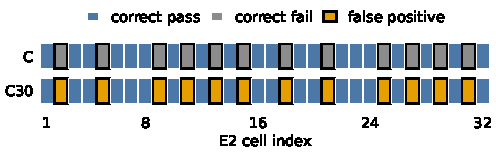
\includegraphics[width=0.98\linewidth]{figures/fig5_e2_fidelity_strip.pdf}
\caption{Replay-to-deployment feasibility for all 32 E2 cells. Blue and gray
tiles are correct pass/fail directions; orange tiles are C30 false positives.
Black outlines mark cells that physically fail P1+.}
\label{fig:e2strip}
\end{figure}

Three PPO arms pass all six physical repeats: C-1, C30-1, and
C30-2; both all2 anchors also pass. The three feasible PPO arms have
scenario costs 42.8--50.5\% below all2, but this comparison is conditional on
the declared ledger and synthetic API sink. C-2 is a decisive negative case:
it averages only 4--7 on-time offline requests out of 120 and leaves about 80
unfinished, despite lower cost. C30-3 is a sharper boundary: it completes
the offline stream eventually, but roughly 11 of 120 offline requests miss their
deadline per repeat, so its lower cost is not feasible saving. Online requests are
on time in every cell; the E2 failures
are therefore isolated to the offline deadline path rather than hidden by an
online regression.

Predictions were frozen before physical execution. Table~\ref{tab:e2prediction}
compares each cell with its corresponding replay: C correctly predicts all 20
passes and 12 failures, whereas C30 predicts all cells feasible and misses both
negative checkpoints. For each replay model, these 32 comparisons reuse 12
policy/window predictions; the physical repeats are not independent predictions.
The two replay models have window-cost MAE of 0.0804 and 0.4657 scenario USD,
respectively. C-2 exposes a startup--cooldown interaction: the 60\,s cooldown
begins at the capacity-target change. In C30 replay, readiness
precedes cooldown expiry, leaving time to serve queued work;
in C replay and most physical restarts, readiness follows expiry,
allowing almost immediate scale-down. Across the six physical
C-2 runs, 72 of 73 restarts taking over 60\,s enter draining
within two seconds of readiness (see the supplement's
Retrospective E2 lifecycle diagnosis section).

\begin{table}[t]
\centering
\small
\caption{Frozen replay versus E2 physical outcomes. Agreement counts repeated
physical cells; false positives predict feasibility where P1+ fails.}
\label{tab:e2prediction}
\par\vspace{4pt}
\begin{tabular*}{\linewidth}{@{\extracolsep{\fill}}lrrr@{}}
\toprule
Replay & Agreement & False positives & Cost MAE\\
\midrule
C & 32/32 & 0/12 & 0.0804\\
C30 & 20/32 & 12/12 & 0.4657\\
\bottomrule
\end{tabular*}
\end{table}

The earlier 38-cell Bridge campaign contains rule, guard, and PPO
arms on a separate runtime. C also has higher feasibility agreement and
lower cost MAE there (Table~\ref{tab:crosscampaign}); the campaigns are not pooled.
This repeated agreement motivates testing C as a screening rule on new checkpoints.

\begin{table}[t]
\centering
\small
\caption{Replay-to-deployment agreement and window-cost MAE.
Bridge and E2 include all technically valid cells, including anchors and
deadline failures; E3 includes its 24 policy cells. Agreement compares each
window prediction with repeated physical outcomes. Cost MAE is in scenario USD.}
\label{tab:crosscampaign}
\setlength{\tabcolsep}{3pt}
\par\vspace{4pt}
\begin{tabular*}{\linewidth}{@{\extracolsep{\fill}}llrr@{}}
\toprule
Campaign & Replay & Agreement & Cost MAE\\
\midrule
% Derived from docs/maxopt_v7_bridge_extension_20261002/e1_reconciliation/E1_RECONCILIATION.json.
Bridge replay & 38 & 36/38; 4.06\% & 21/38; 30.3\% \\
Deployment campaign & 32 & 32/32; 0.0804 & 20/32; 0.4657 \\
\bottomrule

\end{tabular*}
\end{table}

Both training environments yield passing and failing E2 checkpoints.
E3 tests whether C's agreement transfers to six previously undeployed
checkpoints. From 90 eligible candidates, C predicts 67 feasible on both known
windows and rejects 23. A fixed ordering selects three distinct trajectories
from each group; C30 does not enter selection. All six pass every physical
run (two windows, two repeats), as do both all2 anchors. C therefore falsely
rejects three feasible candidates, while C30 accepts all six. Across the 24
policy cells, C30 also has lower cost MAE (Table~\ref{tab:crosscampaign}),
reversing the E2 ordering. These selected cases show that earlier agreement
does not establish reliable screening of new checkpoints and execution
conditions; they do not estimate population screening accuracy. The supplement
records candidate selection, predictions, and the separate window allocations.

\subsection{Control case study: feasibility and cost}
The earlier rule-based guard remains the control case for the same contract; E2
extends that contract to frozen learned checkpoints. Table~\ref{tab:feas} summarizes the rule-control case study. All2 and all1 satisfy
the registered completion target. H is technically valid but fails the P1 gate in
all three recovery repeats (116/120, 113/120, and 116/120 offline on time). In
that held-out study, the guard repairs this failure without changing the workload or
the locked model.

\begin{table}[t]
\centering
\small
\caption{Formal held-out results. Each arm has three repeats per window;
H has 15 offline deadline misses across its three recovery repeats.}
\label{tab:feas}
\par\vspace{4pt}
\begin{tabular*}{\linewidth}{@{\extracolsep{\fill}}lccc@{}}
\toprule
Arm & tech. & offline & online\\
\midrule
all2 & 9/9 & 9/9 (120/120) & 9/9\\
all1 & 9/9 & 9/9 (120/120) & 9/9\\
H & 9/9 & 6/9 & 9/9\\
H+guard & 9/9 & 9/9 (120/120) & 9/9\\
\bottomrule
\end{tabular*}
\end{table}



H+guard's window cost is lower than all1 by 21.96\%, 48.19\%, and 58.08\%
in steady, recovery, and burst-offline, respectively. Their equal-window mean
is 42.74\%, above the preregistered 25\% P2 line, although steady falls below
that stretch target. Including setup and cleanup gives a separate mean saving
of 38.86\%.

The primary ledger covers the same 2,100 s interval; the deployment ledger also
charges setup and cleanup. The supplementary table retains both views, with
unchanged prices and event streams.

Before execution, E's locked recovery prediction identifies four unfinished
offline requests; the three physical H repeats leave four, seven, and four
unfinished, for 15 total misses. This prediction is interpreted alongside, not
substituted for, the observed completion evidence.

\subsection{Latency--cost trade-off}
The saving has a visible online latency price. The supplementary tail table reports each
repeat's online p99 rather than a pooled average. The always-on references remain
near 1.6--2.6 s, while both dynamic arms reach about 15--19 s because requests can
wait for the 10 s routing path and the synthetic API sink. The guard's role is
deadline protection for offline work; it does not remove this routing delay. Every
observed p99 remains below the registered 60 s online deadline, so the result is an
explicit SLO-margin-for-cost trade-off.

\subsection{Guard activation and mechanism}
The guard checks deadline risk using the visible queue, running-job ages,
lifecycle delay, and concurrency-four service estimate. Equation~\ref{eq:guard-update} retains risk IDs until dispatch
or removal from the pending queue and distinguishes risk from a target raise.
For the earlier guard case study, the formal logs contain 59 risk-active ticks, all in recovery:
the guard raised the target above H twice, with the remaining risk ticks maintaining
the already-raised target. No risk-active tick occurred in steady or burst-offline.
Per-repeat counts and slack ranges are shown in Table~\ref{tab:guard}.

\begin{table}[t]
\centering
\small
\caption{Guard activity by recovery repeat. Ticks are window seconds; slack is
the minimum pending-offline time to deadline (seconds), before subtracting
service time.}
\label{tab:guard}
\par\vspace{4pt}
\begin{tabular*}{\linewidth}{@{\extracolsep{\fill}}lrrrr@{}}
\toprule
Repeat & risk ticks & target raises & tick range & slack range\\
\midrule
1 & 30 & 1 & 1982--2011 & 29--58 \\
2 & 0 & 0 & -- & -- \\
3 & 29 & 1 & 2027--2055 & 30--58 \\
\bottomrule

\end{tabular*}
\end{table}

\begin{figure*}[t]
\centering
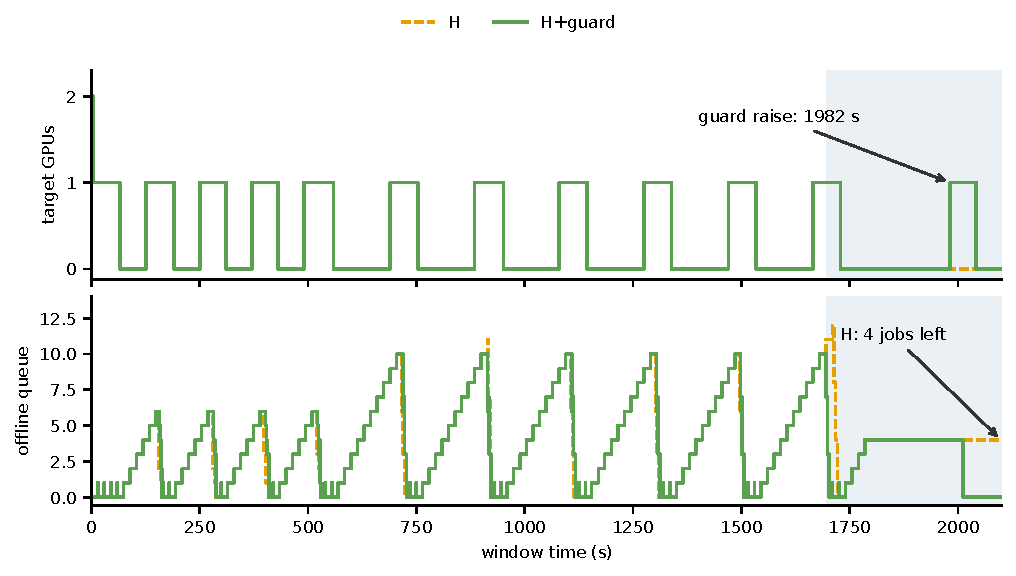
\includegraphics[width=0.96\linewidth]{figures/fig4_recovery_timeline.pdf}
\caption{Recovery target and offline queue in repeat 1. The shaded final interval
contains the guard raise at 1982 s; H leaves four offline jobs queued, while
the guard clears them. Across all three H repeats, 15 jobs miss their deadlines.}
\end{figure*}

\subsection{Price sensitivity}
We reprice H+guard and all1 over 27 window--GPU--API price combinations,
keeping their event streams fixed. At the reference prices the
three window savings are 21.96\%, 48.19\%, and 58.08\%; the sign can reverse when
GPU capacity is cheap and API use is expensive. The only negative cell is steady
at GPU multiplier 0.5 and API multiplier 2.0, where savings are $-39.59\%$. The
steady break-even API multiplier at half-price GPUs is 1.004. Recovery and burst
remain positive across the tested grid, but this is a finite sensitivity analysis,
not a provider billing forecast.

\begin{table}[t]
\centering
\small
\caption{Price-grid savings (percent) for API multipliers 0.5/1.0/2.0. Rows are
GPU multipliers 0.5/1.0/2.0; the final column is the break-even API multiplier.}
\label{tab:prices}
\par\vspace{4pt}
\begin{tabular*}{\linewidth}{@{\extracolsep{\fill}}llrrr r@{}}
\toprule
Window & GPU & API .5 & API 1 & API 2 & break-even\\
\midrule
steady & 0.5 & 20.05 & 0.17 & -39.59 & 1.004 \\
steady & 1.0 & 31.90 & 21.96 & 2.07 & 2.104 \\
steady & 2.0 & 37.84 & 32.86 & 22.92 & 4.304 \\
recovery & 0.5 & 46.51 & 41.13 & 30.37 & 4.822 \\
recovery & 1.0 & 50.88 & 48.19 & 42.81 & 9.953 \\
recovery & 2.0 & 53.07 & 51.73 & 49.04 & 20.216 \\
burst-offline & 0.5 & 56.53 & 53.75 & 48.18 & 10.647 \\
burst-offline & 1.0 & 59.47 & 58.08 & 55.29 & 21.841 \\
burst-offline & 2.0 & 60.95 & 60.25 & 58.86 & 44.227 \\
\bottomrule

\end{tabular*}
\end{table}

External checks evaluate three implemented rule baselines: queue-target scaling
(B-HPA), Holt queue prediction (B-PRED), and queueing-based capacity selection
(B-MMC). Each meets all deadlines in its nine formal runs. A separate same-runtime
comparison finds lower H+guard cost than B-HPA on two known Qwen windows, with
higher API share and queue exposure. These results and the Llama and load-boundary
studies bound the guard's scope; they are not additional E2 samples. Full results
and baseline definitions appear in the supplement's External-validity evidence
section.

\section{Discussion}
FidelityLoop aims to assess whether a scheduling policy will meet deadlines
in physical execution and, if so, what resource use and cost it will incur.
This requires validating request timing, capacity availability, and resource
accounting together; improving one metric alone is insufficient.
For example, C30's startup correction reduced resource-prediction error
under fixed H, yet C predicted feasibility more accurately in Bridge and E2.
E3 then reverses the comparison: C rejects three feasible new checkpoints.
An evaluator must therefore be checked on the deployment it is meant to screen.

\subsection{Validating predictions across levels}
Better local-service fit can accompany worse closed-loop resource prediction.
The startup-endpoint comparison identifies one source of this gap, while the
trajectory analysis shows that aggregate occupied-resource errors can hide
temporal misalignment. Validation should therefore distinguish setup from
window scale-out and check states, actions, and occupied resources alongside
matched-service error.

The guard shows how a controller can act on deadline risk from observed queues
and frozen safety estimates. It repairs H's held-out recovery failure, but H
does not read the simulator's startup parameters: the endpoint correction and
the guard benefit have distinct causal roles.

\subsection{Resource and latency trade-offs}
The elastic policies trade online latency margin for lower occupied capacity:
meeting the 60-second SLO can still leave excessive tail latency.
The steady-window cost reversal at half-price GPUs and high API prices
also shows that policy choice depends on the accounting assumptions.

The same-runtime baseline comparison makes this trade-off explicit. On two known Qwen
inputs, H+guard lowers cost relative to B-HPA while increasing synthetic-API
share, lifecycle-event counts, and queue exposure. The comparison evaluates
complete policies, including their dispatch rules. The Llama deadline miss
and the failed higher-intensity Azure capacity tests show where the successful
Qwen outcome stops transferring. On the first feasible tested Azure intensity,
most savings occur in the final 600 seconds.

The supplementary CPU microbenchmark times \texttt{adapter.decide} on
reconstructed states outside live serving. It measures decision-call latency,
not full-controller or end-to-end overhead.

\section{Limitations and negative results}
The synthetic API uses a five-second timer and a routing wait; it does not generate
or evaluate an answer. Consequently, the cost result is a controlled resource
contract, not a claim that a commercial API can replace local serving at equal
quality. GPU off is verified process and resource release, not physical power-off,
energy measurement, or a cloud provider bill. The three windows are cases rather
than independent workloads, and the three repeats support engineering robustness,
not broad statistical generalization.

H's recovery misses show that economical cooldown decisions can leave offline
work unfinished. The guard repairs the observed case without a general safety
guarantee. The historical V--E comparison remains confounded by deployment drift;
later refitting and policy comparisons do not isolate its calibration effect.

E2 covers two A100 devices, one Qwen model, two windows, and five frozen
checkpoints. It establishes neither heterogeneous-device scalability nor a
general ranking of PPO training environments or PPO versus the guard. The
38-cell Bridge campaign uses a separate runtime and is not pooled with E2.
E3 adds six nonrandom checkpoints from two training seeds on known windows,
with one allocation per window; checkpoint and execution-condition effects
are not isolated. Its all-feasible cohort cannot measure detection of
infeasible deployments or establish a generally superior replay model.
Llama adds one similarly sized family and two repeats, including a guarded
deadline failure; broader model scales, quantization, and engines remain untested.
The same-runtime baseline compares two complete policies on known Qwen inputs,
so it neither adds held-out workloads nor isolates the guard inside the other
controllers. Candidate families and workloads were locked before replay, with
no window replacement. Missing session identities and regular offline pressure
limit population-level inference. CPU verification covers all accepted records. A recovery addendum restores
the root environment snapshot from identical, hash-bound per-run copies;
the original archive checksum sidecar remains unavailable.

\section{Conclusion}
FidelityLoop provides a replayable contract for connecting elastic-serving policy
decisions to lifecycle execution and resource/cost accounting. It shows why
predictions need validation across levels: local-service fit can improve while
resource prediction worsens, and accurate total occupation can hide large
trajectory errors. Startup-endpoint isolation
and event-level counterexamples explain where these checks diverge. Lifecycle
states, control decisions, and resource use should therefore be validated together.

The guard case study quantifies deadline protection and its resource, routing,
and cost trade-offs. E2 extends the same contract to frozen PPO checkpoints: some
checkpoints reduce scenario cost while preserving every deadline, whereas the
negative checkpoints reveal why cost must be conditioned on feasibility.
E3 also exposes false rejections by the replay model that best matched E2.
Under the studied synthetic-API setting, both the candidate policy and its
screening model need deployment validation before predicted savings guide decisions.
